% The format (A5) is selected to facilitate reading on small
% devices and should NOT be changed. 
\documentclass[a5paper,10pt,oneside]{article}

% The package babel is loaded for Swdish with Swedish hyphenation,
% replaces "Contents" with "Innehållsförteckning, "References"
% with "Litteraturförteckning", etc.
\usepackage[swedish]{babel}

\usepackage[T1]{fontenc}

% The package "inputenc" lets us specify what character encoding
% has been used to save the .tex file. If your computer runs
% Linux, the encoding is probably "utf8" by default, while under
% Windows the default will probably be "latin1" The wrong
% character encoding may give strange signs instead of "å", "ä"
% and "ö" or may result in compilation errors.

%\usepackage[latin1]{inputenc} % Probably right if you use Windows
\usepackage[utf8]{inputenc}  % Probably right if you use Linux

% The packages listed below are optional and can be removed if you
% don't use them 
\usepackage{graphicx} 
\usepackage{cite}
\usepackage{url}
\usepackage{ifthen}
\usepackage{listings}	


% These two lines set up options for the listings package and
% can be removed if you don't use it, or changed if you, e.g, 
% use another language than Java. 
% For more information about the listings package see:
% ftp://ftp.tex.ac.uk/tex-archive/macros/latex/contrib/listings/listings.pdf
\def \lstlistingname {Kodexempel}
\lstset{language=Java,tabsize=3,numbers=left,frame=L,floatplacement=hbtp}


\usepackage{ifpdf}
\ifpdf
	\usepackage[hidelinks]{hyperref}
\else
	\usepackage{url}
\fi


% Change NR and TITLE below to appropriate values
\title{Tema NR: 3 Träd}

% Write the name and user namn for all participants in the group here.
% Separate persons with \and
\author{Oscar Törnquist \url{osta3589} \and Emil Rosell \url{emro9957}}



\begin{document}
\maketitle

\section*{Enkelrotationer}

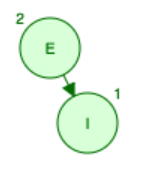
\includegraphics[scale=0.4]{em}
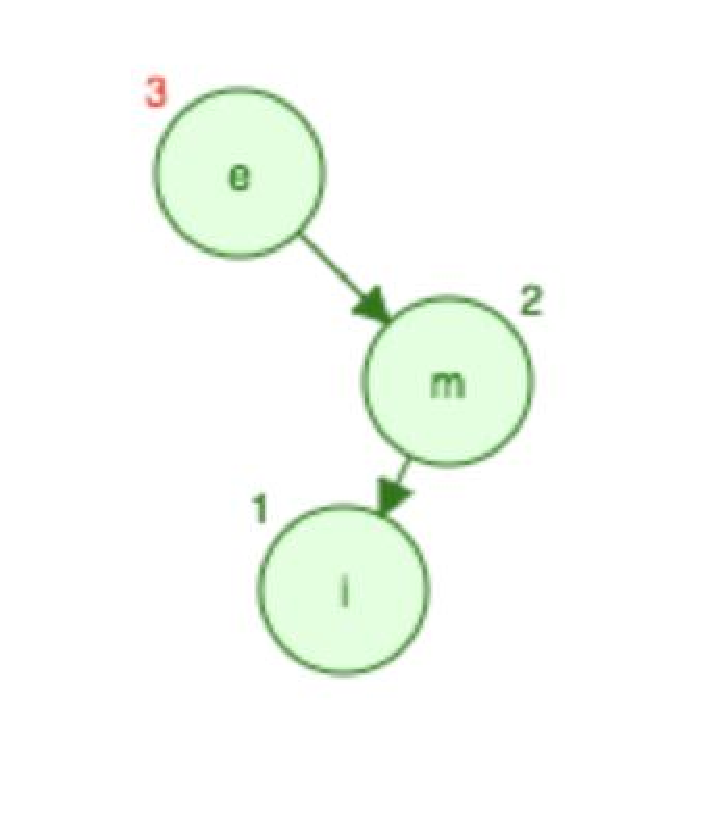
\includegraphics[scale=0.4]{emiBefore}
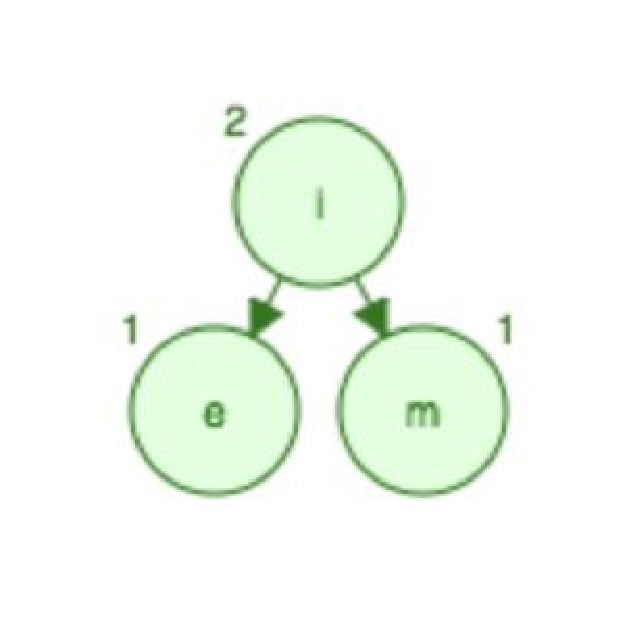
\includegraphics[scale=0.5]{emiAfter}

Enkelrotationer är den mindre komplexa rotationssorten för AVL-träd. När en en nod har subträd som vars djup skiljer sig med mer än ett behövs det balanseras upp vilket är rotationernas jobb. För att börja med ett simpelt exempel så har vi använt oss av bokstäverna $E, I $ och $M$. Vi börjar med att lägga till roten i det binära sökträdet, i det här fallet är det ett $E$, därefter lägger vi till ett $I$ som är större än $E$ och läggs därför till höger i ett subträd till roten. Om vi sen ska lägga till ett $M$ till trädet så är det större än båda noderna som tidigare lagts till vilket betyder att $M$'et läggs till som ett barn till noden $I$. När kontrollen sen sker om balansen upprätthålls så börjar kontrollen i den noden som senast lades till, kontrollen förflyttas till föräldern till den tidigare noden och upptäcker att det högra subträdet har djupet 1 medans det vänsta har djupet 0 vilket är fullt tillåtet då skillnaden inte får vara större än 1. När kontrollen sen kommer upp till roten så kontrolleras subträden och skillnaden är då mer än 1, närmare bestämt är djupet på vänstra subträdet 0 och högra 2. För att åtgärda balansen i trädet så flyttas noden till höger om roten, i detta fall $I$, ett steg åt vänster. Den tidigare roten är nu en barnnod till noden som tidigare låg som ett barn i höger subträd. Enkelrotationen har löst balansen med ett steg där obalansen låg i roten. 

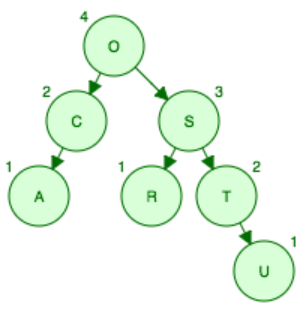
\includegraphics[scale=0.3]{advEnk}
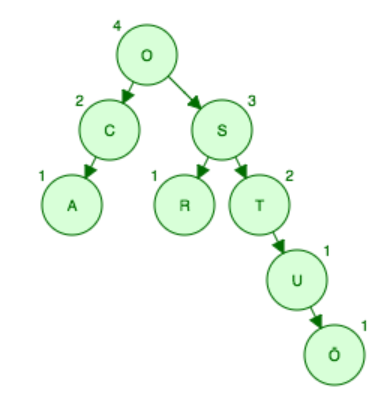
\includegraphics[scale=0.3]{advEnkB}
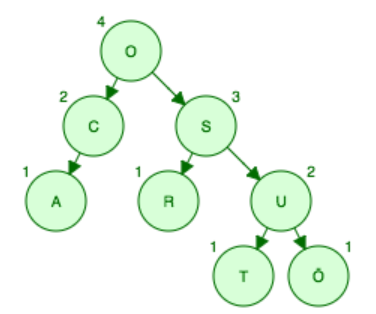
\includegraphics[scale=0.3]{advEnkA}

Enkelrotationer är dock något som inte bara används av rotnoden i trädet utan kan användas av noter som ligger längre ner också. Nästa exempel visar när en enkelrotation sker på ett annat djup än rotens djup. I den första bilden ovanför detta stycke så har vi ett träd av bokstäverna \textit{O-S-C-A-R-T-U}. Den andra bilden visar hur ett $Ö$ läggs till i trädet och när balansen kontrolleras så uppstår det en obalans redan vid $T$-noden. Där är det återigen en skillnad som är större än 1 mellan det högra subträdet och det vänstra, vilket då behöver balanseras med hjälp av enkelrotationen. Sista bilden visar att $U$ flyttar upp ett steg, $T$ läggs som vänstra barnet till $U$ då $T < U$ och $Ö$ hänger bara på när $U$ flyttas upp. 

\section*{Dubbelrotationer}


\end{document}
